\documentclass{article} % For LaTeX2e
\usepackage{iclr2026_conference,times}

\input{math_commands.tex}

\usepackage{hyperref}
\usepackage{graphicx}
\usepackage{booktabs}
\usepackage{amsmath,amssymb}
\usepackage{microtype}
\usepackage{subcaption}
\usepackage{enumitem}
\usepackage{array}
\graphicspath{{figures/}}

\hypersetup{
  colorlinks=true,
  linkcolor=blue,
  citecolor=blue,
  urlcolor=blue
}

\iclrfinalcopy

\title{A Case Study of Staged Metric-Gated GRPO for Visual Numeric Reasoning}

% Keep the real author block in source; the ICLR style will hide it in review mode
% until \iclrfinalcopy is restored.
\author{Kunal Ghosh\\
Purdue University\\
West Lafayette, Indiana, USA\\
\texttt{ghosh178@purdue.edu}\\
\texttt{kg.aero@gmail.com}}

\newcommand{\mcell}[1]{\begin{tabular}[t]{@{}l@{}}#1\end{tabular}}

\begin{document}

\maketitle
\fancyhead{}
\lhead{}
\chead{}
\rhead{}

\begin{abstract}
We present a staged metric-gated GRPO fine-tuning pipeline for visual numeric reasoning. The pipeline combines four components: a phase-wise curriculum over filtered MathVista subsets, a strict \texttt{<REASONING>} / \texttt{<SOLUTION>} response contract, a checkpoint-metric controller that preserves structure-oriented reward floors under formatting or completion degradation and increases correctness weight after structural metrics stabilize and exact-match progress stalls, and alias-based checkpoint selection to address non-monotonic checkpoint quality. The resulting trajectory follows a consistent two-stage progression: smoke-phase runs on \texttt{testmini} stabilize parseability and output structure, and larger-split Phase C fine-tuning on \texttt{test}, evaluated on \texttt{testmini}, delivers the main correctness improvement. Under the checkpoint-side evaluation protocol used for continuation, the best large Phase C checkpoint and the best dedicated Phase D checkpoint each achieve exact-match and tolerance accuracy of 0.75, compared with 0.375 for a pre-refactor baseline, while maintaining parseability 1.0 and zero truncation on the monitored subset. These results indicate that curriculum filtering, metric-gated reward adaptation, and checkpoint-aware continuation support a stable, structure-first RL fine-tuning pipeline for multimodal numeric question answering under constrained compute.

\textbf{Code:} \url{https://github.com/kgaero/RL_GSPO_Qwen2.5VLM}
\end{abstract}

\section{Introduction}

Reinforcement-learning fine-tuning for language and vision-language models is often summarized as a direct mapping from reward design to improved accuracy. In multimodal settings, however, the optimization problem is more complex \citep{yuan2025vlcogito}. Before correctness reward becomes informative, the policy must already emit outputs that are parseable, non-truncated, and structurally compatible with the evaluator \citep{shen2025satori}. If those preconditions are unstable, RL updates can be difficult to interpret because an apparent correctness failure may in fact be a formatting or completion failure \citep{shen2025satori}.

This paper investigates a staged metric-gated GRPO fine-tuning pipeline for visual numeric reasoning using \texttt{Qwen2.5-VL-7B-Instruct} as the base VLM. The pipeline leaves the GRPO objective unchanged and augments fine-tuning with filtered curriculum stages, a strict response contract, rule-based reward adaptation keyed to checkpoint metrics, and checkpoint aliases that allow continuation from the best structural or composite checkpoint rather than always from the most recent one. We analyze how this fine-tuning pipeline produces a structure-first and correctness-later trajectory for multimodal numeric question answering.

The implementation is designed to be auditable: controller states are saved, checkpoint aliases are explicit, reward weights are persisted, and the main milestones are recoverable from checkpoint-side evaluation logs. This instrumentation is valuable in constrained-compute RL settings, where structural failures dominate early training and continuation decisions materially affect outcomes.

Figure~\ref{fig:pipeline} summarizes the loop. A base VLM is prepared with LoRA adapters, fine-tuned on a stage-filtered phase mixture, evaluated checkpoint by checkpoint, and then fed back into a controller that updates reward weights after each checkpoint evaluation. Table~\ref{tab:stage-matrix} shows that the curriculum is implemented as overlapping filtered views over the same MathVista split rather than as disjoint datasets.

\paragraph{Contributions.}
\begin{enumerate}[leftmargin=1.2em]
\item We document a staged GRPO fine-tuning pipeline for visual numeric reasoning that explicitly prioritizes structure stabilization before the main correctness gains.
\item We formalize the metric-gated reward controller and checkpoint aliasing logic so they can be read as an auditable algorithm rather than as scattered implementation details.
\item We characterize the checkpoint-side training trajectory used for continuation decisions, including the 0.75 exact-match milestone reached by the best large Phase C and dedicated Phase D checkpoints.
\end{enumerate}

\begin{figure}[t]
\centering
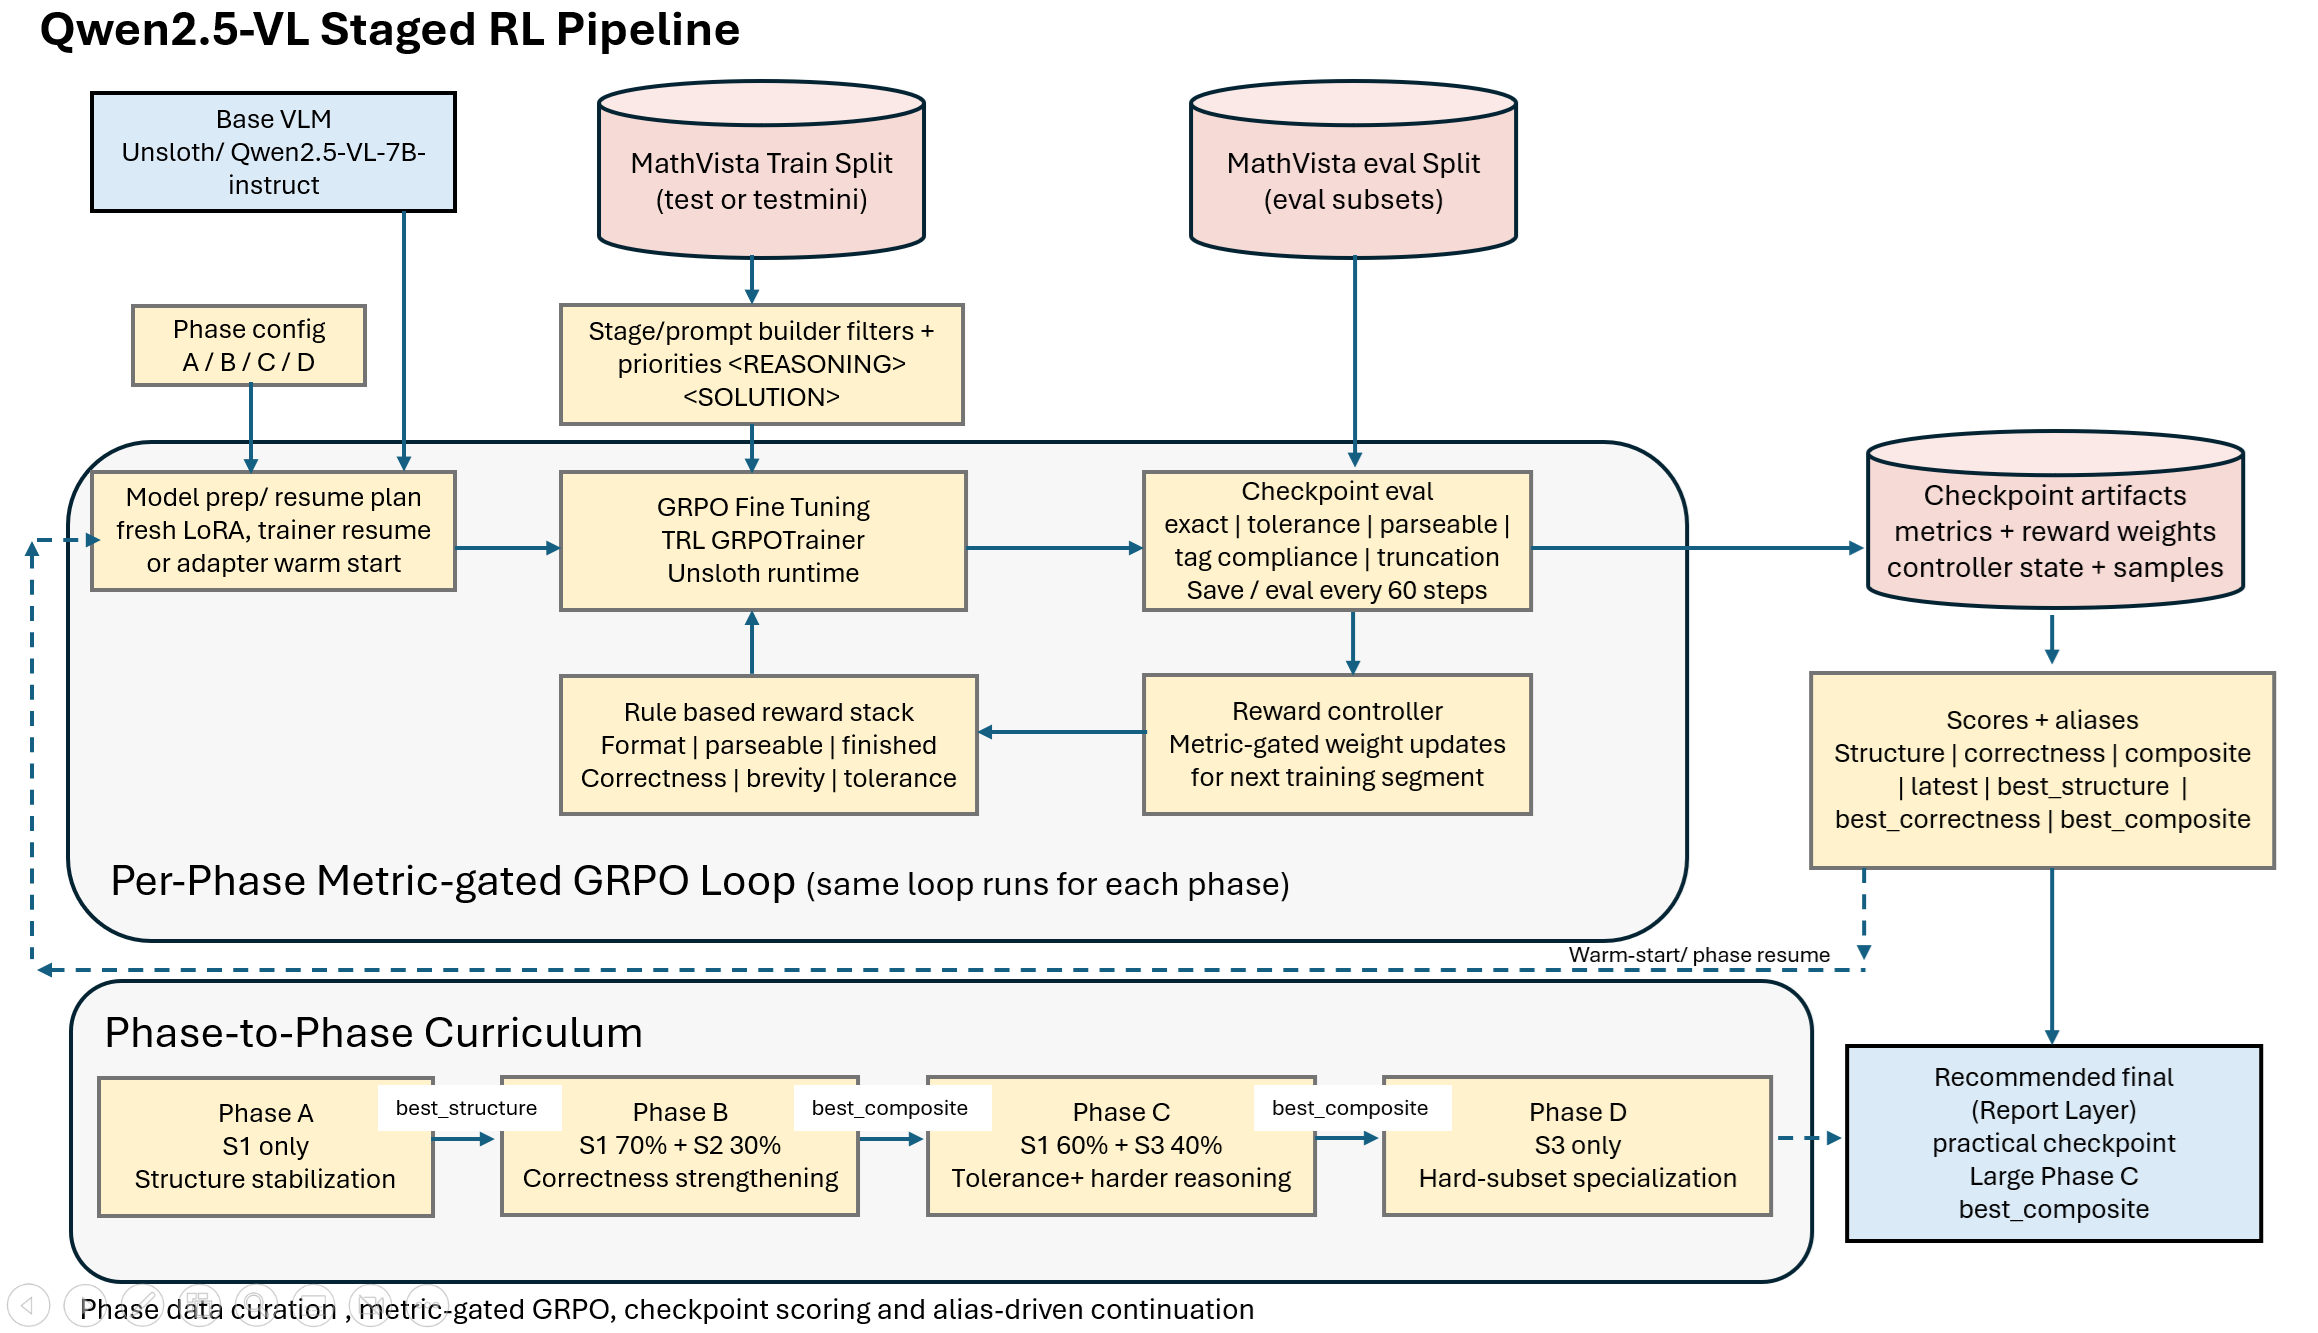
\includegraphics[width=\linewidth]{staged_training_pipeline_better.png}
\caption{Overview of the staged metric-gated GRPO loop. The pipeline couples phase-specific data curation, GRPO fine-tuning, checkpoint-side evaluation, reward-weight adaptation, and alias-based continuation. The method studied here is the fine-tuning pipeline around GRPO rather than a new GRPO loss.}
\label{fig:pipeline}
\end{figure}

\section{Related Work}

\paragraph{RL fine-tuning and preference optimization.}
Recent RLHF and preference-optimization work has primarily focused on new objectives or more efficient learning regimes. DeepSeekMath introduced GRPO as a group-relative alternative to PPO for mathematical reasoning \citep{deepseekmath2024}. SPPO and Asynchronous RLHF studied, respectively, self-play preference optimization and faster off-policy online RLHF \citep{wu2025sppo,noukhovitch2025async}. More recent multimodal post-training studies have adapted GRPO- or RL-style optimization to vision-language reasoning through cold-start supervision, staged reinforcement learning, and explicit reasoning incentives \citep{huang2025visionr1,wei2025coldstart,chen2025revisualr1}. Our contribution is complementary: we leave the underlying GRPO objective unchanged and study how a staged fine-tuning pipeline combines GRPO with curriculum scheduling, metric-gated reward adaptation, and checkpoint-selection logic in a failure-prone multimodal setting.

\paragraph{Multimodal mathematical reasoning.}
MathVista highlights the difficulty of mathematical reasoning in visual contexts and serves as a benchmark for diagram, chart, table, and numeric question answering behavior \citep{lu2024mathvista}. Recent work has addressed this problem with larger synthetic corpora, progressive curricula, staged reinforcement learning, or more explicit visual reasoning mechanisms \citep{zhang2025mavis,qi2025cogcom,liu2025infimmr,yuan2025vlcogito}. This paper focuses on the training-system side of the problem: a standard pretrained VLM paired with staged curricula, metric-gated reward control, and checkpoint-aware continuation that prioritize structural reliability before stronger correctness pressure.

\paragraph{Curriculum and adaptive reward control.}
Our approach is closest in spirit to curriculum and adaptive-control approaches that treat fine-tuning as a sequence of regimes rather than as one stationary objective. Recent multimodal reasoning work has explored phased reinforcement learning, progressive curriculum RL, and rubric-based curriculum design as mechanisms for stabilizing difficult reasoning behavior \citep{liu2025infimmr,yuan2025vlcogito,chen2026rucl}. The distinctive feature here is the granularity of adaptation: checkpoint metrics trigger reward changes directly within the fine-tuning pipeline.

\section{Problem Setup and Design Goals}

We study a policy $\pi_\theta(c \mid x)$ that maps a visual question-answering input $x$ to a completion $c$. Our method does not treat success as a single scalar notion of accuracy. Instead, it decomposes success into a sequence of preconditions:
\begin{enumerate}[leftmargin=1.2em]
\item the model must emit the required tagged structure,
\item the final answer must be parseable,
\item the answer must finish within the completion budget, and
\item the parsed answer must be correct under exact or tolerance-based matching.
\end{enumerate}
The central question is therefore not only how to optimize correctness, but also when correctness reward becomes informative enough to emphasize. If structure is unstable, correctness reward is sparse because malformed or truncated outputs never reach a meaningful matching stage.

The implementation makes three concrete design choices.
\begin{itemize}[leftmargin=1.2em]
\item \textbf{Easy-to-hard data staging.} The policy first sees easier integer-valued numeric problems before harder float and geometry-heavy subsets are emphasized.
\item \textbf{Metric-gated rewards.} Reward weights change only after checkpoint evaluation, using measured failure modes rather than a fixed epoch schedule.
\item \textbf{Alias-based continuation.} Checkpoint continuation is based on structure, correctness, or composite aliases rather than assuming the latest checkpoint is best.
\end{itemize}
Taken together, these choices define the central design logic of the method.

\section{Method}

\subsection{Task, response contract, and phase structure}

The code targets MathVista-style visual question answering in which the answer is primarily numeric and free-form. Each prompt is wrapped with a strict output contract:
\begin{quote}
\small\ttfamily
<REASONING> ... </REASONING>\\
<SOLUTION> single numeric answer </SOLUTION>
\end{quote}
This contract matters because both the reward functions and the evaluator depend on extracting a unique solution string from the completion. The pipeline also contains a separate multi-choice scaffold, but that branch is disabled by default and is not part of the main evidence.

The curriculum is organized into stages and phases. Stages are filtered subsets over the same dataset. In the default configuration:
\begin{itemize}[leftmargin=1.2em]
\item \textbf{Stage 1} restricts to easier English free-form integer questions on synthetic scenes, tables, and natural images.
\item \textbf{Stage 2} broadens to integer and float answers, adding tables, charts, plots, and scientific figures.
\item \textbf{Stage 3} emphasizes harder geometry, scientific-figure, plot, and abstract-scene problems.
\end{itemize}
Phases then mix these stages with different reward emphases:
\begin{itemize}[leftmargin=1.2em]
\item \textbf{Phase A}: Stage 1 only, structure stabilization.
\item \textbf{Phase B}: $0.7$ Stage 1 + $0.3$ Stage 2, early correctness strengthening.
\item \textbf{Phase C}: $0.6$ Stage 2 + $0.4$ Stage 3, harder reasoning and tolerance reward.
\item \textbf{Phase D}: Stage 3 only, hard-subset specialization with a longer completion budget.
\end{itemize}

\begin{table}[t]
\centering
\setlength{\tabcolsep}{2pt}
\renewcommand{\arraystretch}{1.12}
\scriptsize
\begin{tabular}{>{\raggedright\arraybackslash}p{0.14\linewidth}>{\raggedright\arraybackslash}p{0.27\linewidth}>{\raggedright\arraybackslash}p{0.27\linewidth}>{\raggedright\arraybackslash}p{0.27\linewidth}}
\hline
\textbf{Filter} & \textbf{S1 Easy Numeric} & \textbf{S2 Medium / Float} & \textbf{S3 Hard Numeric} \\
\hline
Stage ID & \texttt{stage1\_easy\_numeric} & \texttt{stage2\_float\_numeric} & \texttt{stage3\_hard\_numeric} \\
\hline
Goal & easy numeric stabilization & moderate precision and broader numeric coverage & harder multistep numeric reasoning \\
\hline
Question type & \texttt{free\_form} & \texttt{free\_form} & \texttt{free\_form} \\
\hline
Answer type & \texttt{integer} & \texttt{integer}, \texttt{float} & \texttt{integer}, \texttt{float} \\
\hline
Language & \texttt{english} & \texttt{english} & \texttt{english} \\
\hline
Answer mode & \texttt{numeric\_free\_form} & \texttt{numeric\_free\_form} & \texttt{numeric\_free\_form} \\
\hline
Context families & \mcell{\texttt{synthetic scene}\\\texttt{table}\\\texttt{natural image}} & \mcell{\texttt{table}\\\texttt{chart}\\\texttt{plot}\\\texttt{scientific figure}\\\texttt{natural image}} & \mcell{\texttt{geometry diagram}\\\texttt{plot}\\\texttt{scientific figure}\\\texttt{abstract scene}} \\
\hline
Skills (any) & \mcell{\texttt{arithmetic reasoning}\\\texttt{statistical reasoning}\\\texttt{numeric commonsense}} & \mcell{\texttt{arithmetic reasoning}\\\texttt{statistical reasoning}\\\texttt{scientific reasoning}\\\texttt{numeric commonsense}} & \mcell{\texttt{geometry reasoning}\\\texttt{algebraic reasoning}\\\texttt{scientific reasoning}\\\texttt{arithmetic reasoning}\\\texttt{statistical reasoning}} \\
\hline
Hard only & False & False & True \\
\hline
Priority bias & \mcell{ctx: synthetic scene\\ctx: table\\skills: arithmetic reasoning\\skills: statistical reasoning\\skills: numeric commonsense\\grades: elementary school\\grades: daily life} & \mcell{ctx: table\\ctx: chart\\ctx: plot\\ctx: scientific figure\\skills: statistical reasoning\\skills: scientific reasoning\\skills: arithmetic reasoning} & \mcell{ctx: geometry diagram\\ctx: scientific figure\\ctx: plot\\skills: geometry reasoning\\skills: algebraic reasoning\\skills: scientific reasoning\\grades: high school\\grades: college} \\
\hline
\end{tabular}
\caption{Code-derived filter definitions for the three numeric curriculum stages used in the main training path. The stages overlap and are implemented as filtered views over the same MathVista split, not as fixed disjoint datasets.}
\label{tab:stage-matrix}
\end{table}

\subsection{Reward decomposition}

For a completion $c$, the method computes six per-sample reward components:
\begin{equation}
R(c)=\sum_{j=1}^{6} w_j r_j(c),
\end{equation}
where the components correspond to \texttt{format}, \texttt{parseable}, \texttt{finished}, \texttt{correctness}, \texttt{brevity}, and \texttt{tolerance}. The initial weights are phase-specific. Phase A places relatively high weight on structure and completion; Phase C raises correctness and activates tolerance reward.

The implementation never allows structure rewards to decay fully to zero. The guiding design principle is that, even when exact match becomes the main target, structural validity remains a necessary condition for receiving informative reward. The exact code-aligned reward definitions are reproduced in the supplement.

\subsection{Metric-gated reward control}

The reward controller updates weights after each checkpoint evaluation using explicit rules derived from observed metrics. Let $p$ denote parseable-answer rate, $s$ solution-tag compliance, $r$ reasoning-tag compliance, $m$ malformed rate, $t$ truncation rate, and $e$ exact match. The controller applies the following guards:
\begin{align}
p < 0.85 &\Rightarrow w_{\text{parseable}} \leftarrow \max(w_{\text{parseable}}, 0.75),\\
(s < 0.90)\ \vee\ (r < 0.88)\ \vee\ (m > 0.10) &\Rightarrow w_{\text{format}} \leftarrow \max(w_{\text{format}}, 0.75),\\
(t > 0.15)\ \vee\ (\bar{\ell} > 0.85L) &\Rightarrow w_{\text{finished}} \leftarrow w_{\text{finished}} + 0.25,
\end{align}
where $\bar{\ell}$ is average completion length and $L$ is the completion budget.

Correctness is escalated only when structure is already stable. Stability requires
\begin{equation}
p \ge 0.92,\quad s \ge 0.95,\quad r \ge 0.93,\quad m \le 0.05,\quad t \le 0.08,
\end{equation}
for a two-checkpoint window. If that condition holds and exact-match improvement over the window is below $0.02$, the controller increases correctness weight by $0.50$. All weights are then clamped to configured bounds. The rule set is intentionally simple enough to audit directly in saved checkpoint artifacts.

\subsection{Checkpoint-side evaluation and alias-based selection}

Instead of treating the most recent checkpoint as the default continuation point, the pipeline evaluates every saved checkpoint and computes three aggregate scores:
\begin{align}
S_{\text{struct}} &= 0.35\,p + 0.20\,s + 0.20\,r - 0.15\,m - 0.10\,t, \\
S_{\text{corr}} &= 0.70\,e + 0.20\,a_{\text{tol}} + 0.10\,p, \\
S_{\text{comp}} &= 0.45\,e + 0.15\,a_{\text{tol}} + 0.15\,p + 0.10\,s + 0.05\,r - 0.05\,m - 0.05\,t,
\end{align}
where $a_{\text{tol}}$ is tolerance accuracy. These scores back four aliases: \texttt{latest}, \texttt{best\_structure}, \texttt{best\_correctness}, and \texttt{best\_composite}. Cross-phase continuation typically resumes from \texttt{best\_structure} or \texttt{best\_composite}, while same-phase restarts may use full trainer resume from \texttt{latest}. This distinction is important in the implementation because the code supports both full trainer-state restoration and LoRA-only warm start.

\section{Experimental Setting and Evaluation Protocol}

\paragraph{Dataset and model.}
We use the Hugging Face release of MathVista\footnote{\url{https://huggingface.co/datasets/AI4Math/MathVista}} and load \texttt{Qwen2.5-VL-7B-Instruct}\footnote{\url{https://huggingface.co/Qwen/Qwen2.5-VL-7B-Instruct}} as the base VLM. For context we cite the MathVista benchmark paper \citep{lu2024mathvista} and the Qwen2.5-VL technical report \citep{bai2025qwen25vl}.

\paragraph{Runtime profile.}
The main reported runs use the conservative \texttt{kaggle\_t4} profile: 4-bit loading, LoRA rank $8$, max sequence length $1280$, image size $336$, gradient accumulation $4$, two sampled generations per prompt during RL fine-tuning, max prompt length $320$, and max completion length $64$ (or $96$ in Phase D). The trainer uses TRL's \texttt{GRPOTrainer} with sequence-level importance sampling and \texttt{dr\_grpo} loss.

\begin{table}[t]
\centering
\setlength{\tabcolsep}{3pt}
\renewcommand{\arraystretch}{1.15}
\scriptsize
\begin{tabular}{>{\raggedright\arraybackslash}p{0.28\linewidth}>{\raggedright\arraybackslash}p{0.12\linewidth}>{\raggedright\arraybackslash}p{0.13\linewidth}>{\raggedright\arraybackslash}p{0.27\linewidth}>{\raggedright\arraybackslash}p{0.10\linewidth}}
\hline
\textbf{Parameter} & \textbf{Default} & \textbf{New Value} & \textbf{Function Name} & \textbf{Phase} \\
\hline
\mcell{\texttt{max\_seq\_length}} & 16384 & 1280 & \mcell{\texttt{FastVisionModel.}\\\texttt{from\_pretrained}} & all \\
\hline
\mcell{\texttt{image\_size}} & 512 & 336 & \mcell{\texttt{build\_stage\_dataset}} & all \\
\hline
\mcell{\texttt{gpu\_memory\_}\\\texttt{utilization}} & 0.8 & 0.65 & \mcell{\texttt{FastVisionModel.}\\\texttt{from\_pretrained}} & all \\
\hline
\mcell{LoRA config\\(\texttt{lora\_rank} / \texttt{max\_lora\_rank} /\\ \texttt{lora\_alpha})} & 16 / None / 16 & 8 / 8 / 8 & \mcell{\texttt{FastVisionModel.}\\\texttt{get\_peft\_model}} & all \\
\hline
\mcell{\texttt{compilation\_}\\\texttt{config}} & unset & \mcell{level 3\\PIECEWISE} & \mcell{\texttt{FastVisionModel.}\\\texttt{from\_pretrained}} & all \\
\hline
\mcell{Training budget\\(\texttt{gradient\_accumulation\_}\\\texttt{steps} /\\ \texttt{num\_generations})} & 2 / 4 & 4 / 2 & \mcell{\texttt{GRPOConfig}} & all \\
\hline
\mcell{Prompt budget\\(\texttt{max\_prompt\_length} /\\ \texttt{max\_completion\_length})} & 1024 / 256 & 320 / 64 & \mcell{\texttt{GRPOConfig}} & A--C, E \\
\hline
\mcell{Eval sampling\\(\texttt{num\_samples\_per\_prompt} /\\ \texttt{max\_eval\_examples\_}\\\texttt{per\_subset})} & 4 / None & 1 / 2 & \mcell{\texttt{SamplingParams}} & all \\
\hline
\mcell{Phase D completion budget\\(\texttt{max\_completion\_length})} & 320 & 96 & \mcell{\texttt{GRPOConfig} /\\\texttt{SamplingParams}} & D only \\
\hline
\end{tabular}
\caption{Code-derived implementation summary of the low-memory profile used by the successful runs. The \textbf{Function Name} column lists the concrete runtime method or config class that consumes the setting, rather than the config-builder that defines its default. The smoke experiments and the larger continuation therefore share the same Kaggle T4-safe operating regime.}
\label{tab:t4-profile}
\end{table}

\paragraph{Checkpoint-side evaluation protocol.}
All quantitative values reported in this paper come from checkpoint-side metrics generated by the code during training and continuation. In the smoke phases, the pipeline trains on \texttt{testmini} and also evaluates on \texttt{testmini} in order to diagnose and correct structural failures efficiently. In the larger continuation, the pipeline trains on \texttt{test} and evaluates on \texttt{testmini}; the headline 0.75 results come from this larger continuation regime and the dedicated Phase D continuation that follows it. Under the Kaggle profile, evaluation uses one sampled completion per prompt and caps each subset at two examples, matching the runtime-constrained operating regime used for the reported runs.

\paragraph{Reproducibility.}
The implementation saves checkpoint-side artifacts including metrics, subset metrics, reward weights, controller state, controller decision logs, prompt-level records, and sample-level JSONL traces. It also includes 28 unit tests covering configuration, data filtering, parsing, checkpointing, evaluation aggregation, controller behavior, and runtime compatibility.

\begin{table}[t]
\centering
\small
\caption{Milestone checkpoints under the checkpoint-side evaluation protocol used by our runs. These are the recorded metrics used by the continuation logic.}
\label{tab:milestones}
\begin{tabular}{lcccccc}
\toprule
Checkpoint & EM & Tol & Parse & Malf. & Trunc. & Comp. \\
\midrule
Pre-refactor baseline & 0.375 & 0.375 & 0.641 & 0.359 & 0.242 & 0.405 \\
Smoke Phase A best & 0.500 & 0.500 & 0.500 & 0.500 & 0.500 & 0.400 \\
Smoke Phase B best & 0.500 & 0.500 & 1.000 & 0.000 & 0.000 & 0.600 \\
Smoke Phase C best & 0.500 & 0.500 & 1.000 & 0.000 & 0.000 & 0.600 \\
Large Phase C best & \textbf{0.750} & \textbf{0.750} & \textbf{1.000} & \textbf{0.000} & \textbf{0.000} & \textbf{0.750} \\
Dedicated Phase D best & \textbf{0.750} & \textbf{0.750} & \textbf{1.000} & \textbf{0.000} & \textbf{0.000} & \textbf{0.750} \\
\bottomrule
\end{tabular}
\end{table}

\section{Results}

\subsection{Structure improves before correctness in the training trajectory}

Table~\ref{tab:milestones} shows the progression most clearly in the checkpoint-side metrics. The pre-refactor baseline reaches only $0.641$ parseability with $0.359$ malformed rate and $0.242$ truncation. Smoke Phase A shortens outputs, but structure remains unstable. A substantial structural transition appears in Smoke Phase B: parseability, reasoning-tag compliance, and solution-tag compliance all reach $1.0$, while malformed outputs and truncation both fall to zero. Exact match, however, remains at $0.5$. These results indicate that the smoke phases on \texttt{testmini} primarily stabilize structure, whereas the larger-split Phase C run on \texttt{test} delivers the main correctness improvement.

\begin{figure*}[p]
\centering

\includegraphics[width=\textwidth,height=0.9\textheight,keepaspectratio]{evolution_panels_notebook_paper.pdf}
\caption{Training evolution across milestone checkpoints. The main qualitative pattern is structure first, correctness later: structural metrics stabilize by the smoke Phase B / Phase C regime, while the 0.75 exact-match milestone appears only after larger continuation.}
\label{fig:evolution}
\end{figure*}

Figure~\ref{fig:evolution} visualizes this transition. Once structural metrics saturate, subsequent progress shifts from improving output validity to improving the correctness of already valid outputs. This interpretation is consistent with the controller design: early checkpoints allocate reward mass to formatting, parseability, and clean completion, whereas later checkpoints inherit those gains and receive greater correctness pressure.

\subsection{The 0.75 milestone appears in larger continuation}

The strongest checkpoints in our runs are the large-split Phase C model at checkpoint 120 and the dedicated Phase D model at checkpoint 130. Relative to the pre-refactor baseline snapshot, the large Phase C checkpoint moves exact match from $0.375$ to $0.75$, tolerance accuracy from $0.375$ to $0.75$, parseability from $0.641$ to $1.0$, and average completion length from $196.3$ to $25.0$ tokens. Table~\ref{tab:base-final} summarizes that before-versus-after comparison.

\begin{table}[t]
\centering
\scriptsize
\setlength{\tabcolsep}{3pt}
\renewcommand{\arraystretch}{1.04}
\caption{Comparison between the pre-refactor baseline snapshot and the best large Phase C checkpoint.}
\label{tab:base-final}
\begin{tabular*}{\linewidth}{@{\extracolsep{\fill}} p{0.50\linewidth} r r r @{}}
\toprule
\multicolumn{4}{@{}l@{}}{\textbf{Core Accuracy}} \\
\cmidrule(lr){1-4}
\textbf{Eval} & \textbf{Base} & \textbf{Trained} & \textbf{\% Improvement} \\
\midrule
\textbf{Exact Match} & \textbf{37.5\%} & \textbf{75.0\%} & \textcolor{green!50!black}{\textbf{+100.0\%}} \\
Tolerance Accuracy & 37.5\% & 75.0\% & \textcolor{green!50!black}{\textbf{+100.0\%}} \\
\midrule
\multicolumn{4}{@{}l@{}}{\textbf{Structure / Completion}} \\
\cmidrule(lr){1-4}
\textbf{Eval} & \textbf{Base} & \textbf{Trained} & \textbf{\% Improvement} \\
\midrule
Parseable Rate & 64.1\% & 100.0\% & \textcolor{green!50!black}{\textbf{+56.1\%}} \\
\textbf{Reasoning Tag Compliance} & \textbf{77.3\%} & \textbf{100.0\%} & \textcolor{green!50!black}{\textbf{+29.3\%}} \\
\textbf{Solution Tag Compliance} & \textbf{75.8\%} & \textbf{100.0\%} & \textcolor{green!50!black}{\textbf{+32.0\%}} \\
Well-Formed Rate & 64.1\% & 100.0\% & \textcolor{green!50!black}{\textbf{+56.1\%}} \\
\mcell{Malformed Rate\\(lower better)} & 35.9\% & 0.0\% & \textcolor{green!50!black}{\textbf{+100.0\%}} \\
Completion Success Rate & 75.8\% & 100.0\% & \textcolor{green!50!black}{\textbf{+32.0\%}} \\
\mcell{Truncation Rate\\(lower better)} & 24.2\% & 0.0\% & \textcolor{green!50!black}{\textbf{+100.0\%}} \\
\midrule
\multicolumn{4}{@{}l@{}}{\textbf{Generation}} \\
\cmidrule(lr){1-4}
\textbf{Eval} & \textbf{Base} & \textbf{Trained} & \textbf{\% Improvement} \\
\midrule
\mcell{Average Completion Tokens\\(lower better)} & 196.3 & 25.0 & \textcolor{green!50!black}{\textbf{+87.3\%}} \\
\mcell{Repetition Rate\\(lower better)} & 10.6\% & 0.0\% & \textcolor{green!50!black}{\textbf{+100.0\%}} \\
Sample Diversity & 32.0\% & 100.0\% & \textcolor{green!50!black}{\textbf{+212.2\%}} \\
\midrule
\multicolumn{4}{@{}l@{}}{\textbf{Scores / Reward}} \\
\cmidrule(lr){1-4}
\textbf{Eval} & \textbf{Base} & \textbf{Trained} & \textbf{\% Improvement} \\
\midrule
Average Total Reward & 3.98 & 6.2 & \textcolor{green!50!black}{\textbf{+55.7\%}} \\
Structure Score & 45.2\% & 75.0\% & \textcolor{green!50!black}{\textbf{+65.8\%}} \\
Correctness Score & 40.2\% & 77.5\% & \textcolor{green!50!black}{\textbf{+93.0\%}} \\
Composite Score & 40.5\% & 75.0\% & \textcolor{green!50!black}{\textbf{+85.0\%}} \\
\bottomrule
\end{tabular*}

\vspace{0.3em}
{\scriptsize\emph{Source:} Pre-Refactor Baseline (\texttt{base}) vs Large Phase C checkpoint-120 (\texttt{lgc:c:120}) from the checkpoint tables generated by the fine-tuning pipeline.}
\end{table}

The dedicated Phase D run matches, rather than exceeds, the best Phase C score. This indicates that hard-subset specialization is a viable continuation path, while the mixed Stage 2/3 continuation remains the strongest route to the 0.75 milestone within the reported runs.

\subsection{Checkpoint-side results motivate alias-based selection}

The checkpoint-side results also clarify the role of alias-based checkpoint selection. In Smoke Phase B, the best composite checkpoint reaches exact match $0.5$ with perfect structure, while the latest checkpoint regresses to exact match $0.0$ despite retaining parseability and tag compliance at $1.0$. In the same-notebook Phase D branch, the best checkpoint reaches $0.75$ exact match but the latest checkpoint ends at $0.5$. This non-monotonicity in the checkpoint lineage explains why explicit aliases are preferable to always resuming from \texttt{latest}.

\subsection{The controller audit is consistent with the intended policy}

The saved controller audit covers 26 evaluated checkpoints across seven phase resets. Its main descriptive result is that the rules fire in the intended order. Parseability, formatting, and finish guards fire only twice each, concentrated in the structurally weak part of the trajectory. Correctness escalation fires 12 times, but only after structure is already stable. Notably, six of those correctness escalations occur on checkpoints where exact match has regressed rather than merely plateaued. This behavior makes the controller's operating bias explicit: once structure is considered stable, the system responds to weak accuracy progress by increasing correctness pressure rather than by re-raising structure rewards.

Figure~\ref{fig:evolution} places that audit trail back into the checkpoint lineage.

\subsection{The 0.75 milestone is obtained under the same low-memory profile}

Table~\ref{tab:t4-profile} and the runtime-tuning tables show that the large continuation does not coincide with a more permissive hardware regime. The successful smoke and large-split runs share the same Kaggle T4 profile: sequence length $1280$ instead of $16384$, image size $336$ instead of $512$, LoRA rank $8$ instead of $16$, and two sampled generations instead of four. The trade-off is a shorter reasoning budget and lower generation diversity. The benefit is a stable single-GPU operating regime that supports both early curriculum validation and later continuation without changing the underlying VRAM regime.

\section{Limitations and Reproducibility}

\begin{itemize}[leftmargin=1.2em]
\item This study was developed and run in a resource-constrained Kaggle T4 environment, and larger-scale experiments are required to determine how far the same curriculum-based RL fine-tuning pipeline stabilizes under longer runs, larger evaluation budgets, and broader hardware regimes.
\item The monitored evaluation subset is tiny in the Kaggle profile, so the quantitative results should be interpreted within that runtime-constrained operating regime.
\item The split protocol is phase-dependent: smoke phases use \texttt{testmini} to rapidly diagnose and stabilize structure, while the main correctness result comes from larger-split Phase C fine-tuning on \texttt{test} with evaluation on \texttt{testmini}.
\item The codebase studies one base model family and one principal hardware profile, and it does not yet include the seed sweeps or controlled ablations needed to validate each component of the fine-tuning pipeline in isolation.
\item The multi-choice branch (Phase E) and multilingual robustness stage are scaffolded but are not part of the main evidence.
\item Even with these limits, the observed structure-first and correctness-later trajectory suggests that curriculum-based staged RL fine-tuning pipelines are a promising research direction for multimodal numeric reasoning and merit further scale-up.
\end{itemize}

The study remains comparatively reproducible. It logs controller decisions at every evaluated checkpoint, persists multiple checkpoint-selection aliases, saves sample-level traces, and includes unit tests for the most failure-prone logic. The supplement expands this record with explicit reward equations, evaluation formulas, controller thresholds, and transfer semantics.

\section{Conclusion}

We presented a staged metric-gated GRPO fine-tuning pipeline for visual numeric reasoning in a resource-constrained setting. The checkpoint-side results indicate a consistent progression: structural validity must become reliable before correctness reward becomes consistently informative. A phase-wise curriculum, metric-gated reward controller, and alias-based checkpoint selection transform a malformed, long-output baseline into checkpoints that reach exact match 0.75 while preserving parseability 1.0 and zero truncation on the monitored subset. Smoke-phase runs stabilize structure on \texttt{testmini}, and larger-split Phase C fine-tuning on \texttt{test} delivers the principal correctness improvement. These findings support staged curriculum-based RL fine-tuning pipelines as a promising direction for multimodal numeric reasoning under practical compute constraints.

\bibliographystyle{iclr2026_conference}
\bibliography{references}

\end{document}
